\begin{abstract}

Recent text-to-image models produce high-quality results but still struggle with precise visual control, balancing multimodal inputs, and demanding extensive training for complex multimodal image generation.
To address these limitations, we propose \textbf{\model}, a novel autoregressive (AR) framework for efficient \textbf{M}ultimodal-condition\textbf{E}d tu\textbf{N}ing for au\textbf{T}\textbf{O}reg\textbf{R}essive multimodal image generation.
% Our paradigm employs a unified AR transformer that processes interleaved visual and textual inputs to generate images autoregressively and deterministically.
% A lightweight multimodal encoder projects inputs into a shared latent sequence, which a single-stream AR decoder then uses to generate image tokens. 
\model combines an AR image generator with a two-stage training paradigm, enabling fine-grained, token-level alignment between multimodal inputs and image outputs—without relying on auxiliary adapters or cross-attention modules.
Central to our method is the two-stage training paradigm: (1) a \textit{multimodal alignment stage} that establishes robust pixel and semantic-level alignment between inputs and generated tokens, followed by (2) a \textit{multimodal instruction tuning stage} that balance model's integration of multimodal inputs and enhance generation controllability.
Extensive experiments demonstrate that, despite a modest model size, suboptimal base components, and limited training resources, \model achieves a strong balance between concept preservation and prompt following on DreamBench++ benchmark, outperforming competitive baselines. 
Additionally, our method also delivers superior image reconstruction fidelity, broad adaptability across multimodal tasks, and an efficient training budget compared to diffusion-based counterparts. 
The dataset, code, and models are available in \href{https://github.com/HaozheZhao/MENTOR}{\texttt{github.com/HaozheZhao/MENTOR}}.
% This work presents an efficient, controllable, and scalable AR pathway for complex multimodal image generation, offering a compelling alternative to prevalent resource-intensive systems.
% 

\begin{figure*}[htbp]
% \vspace{-1ex}
\centering
% 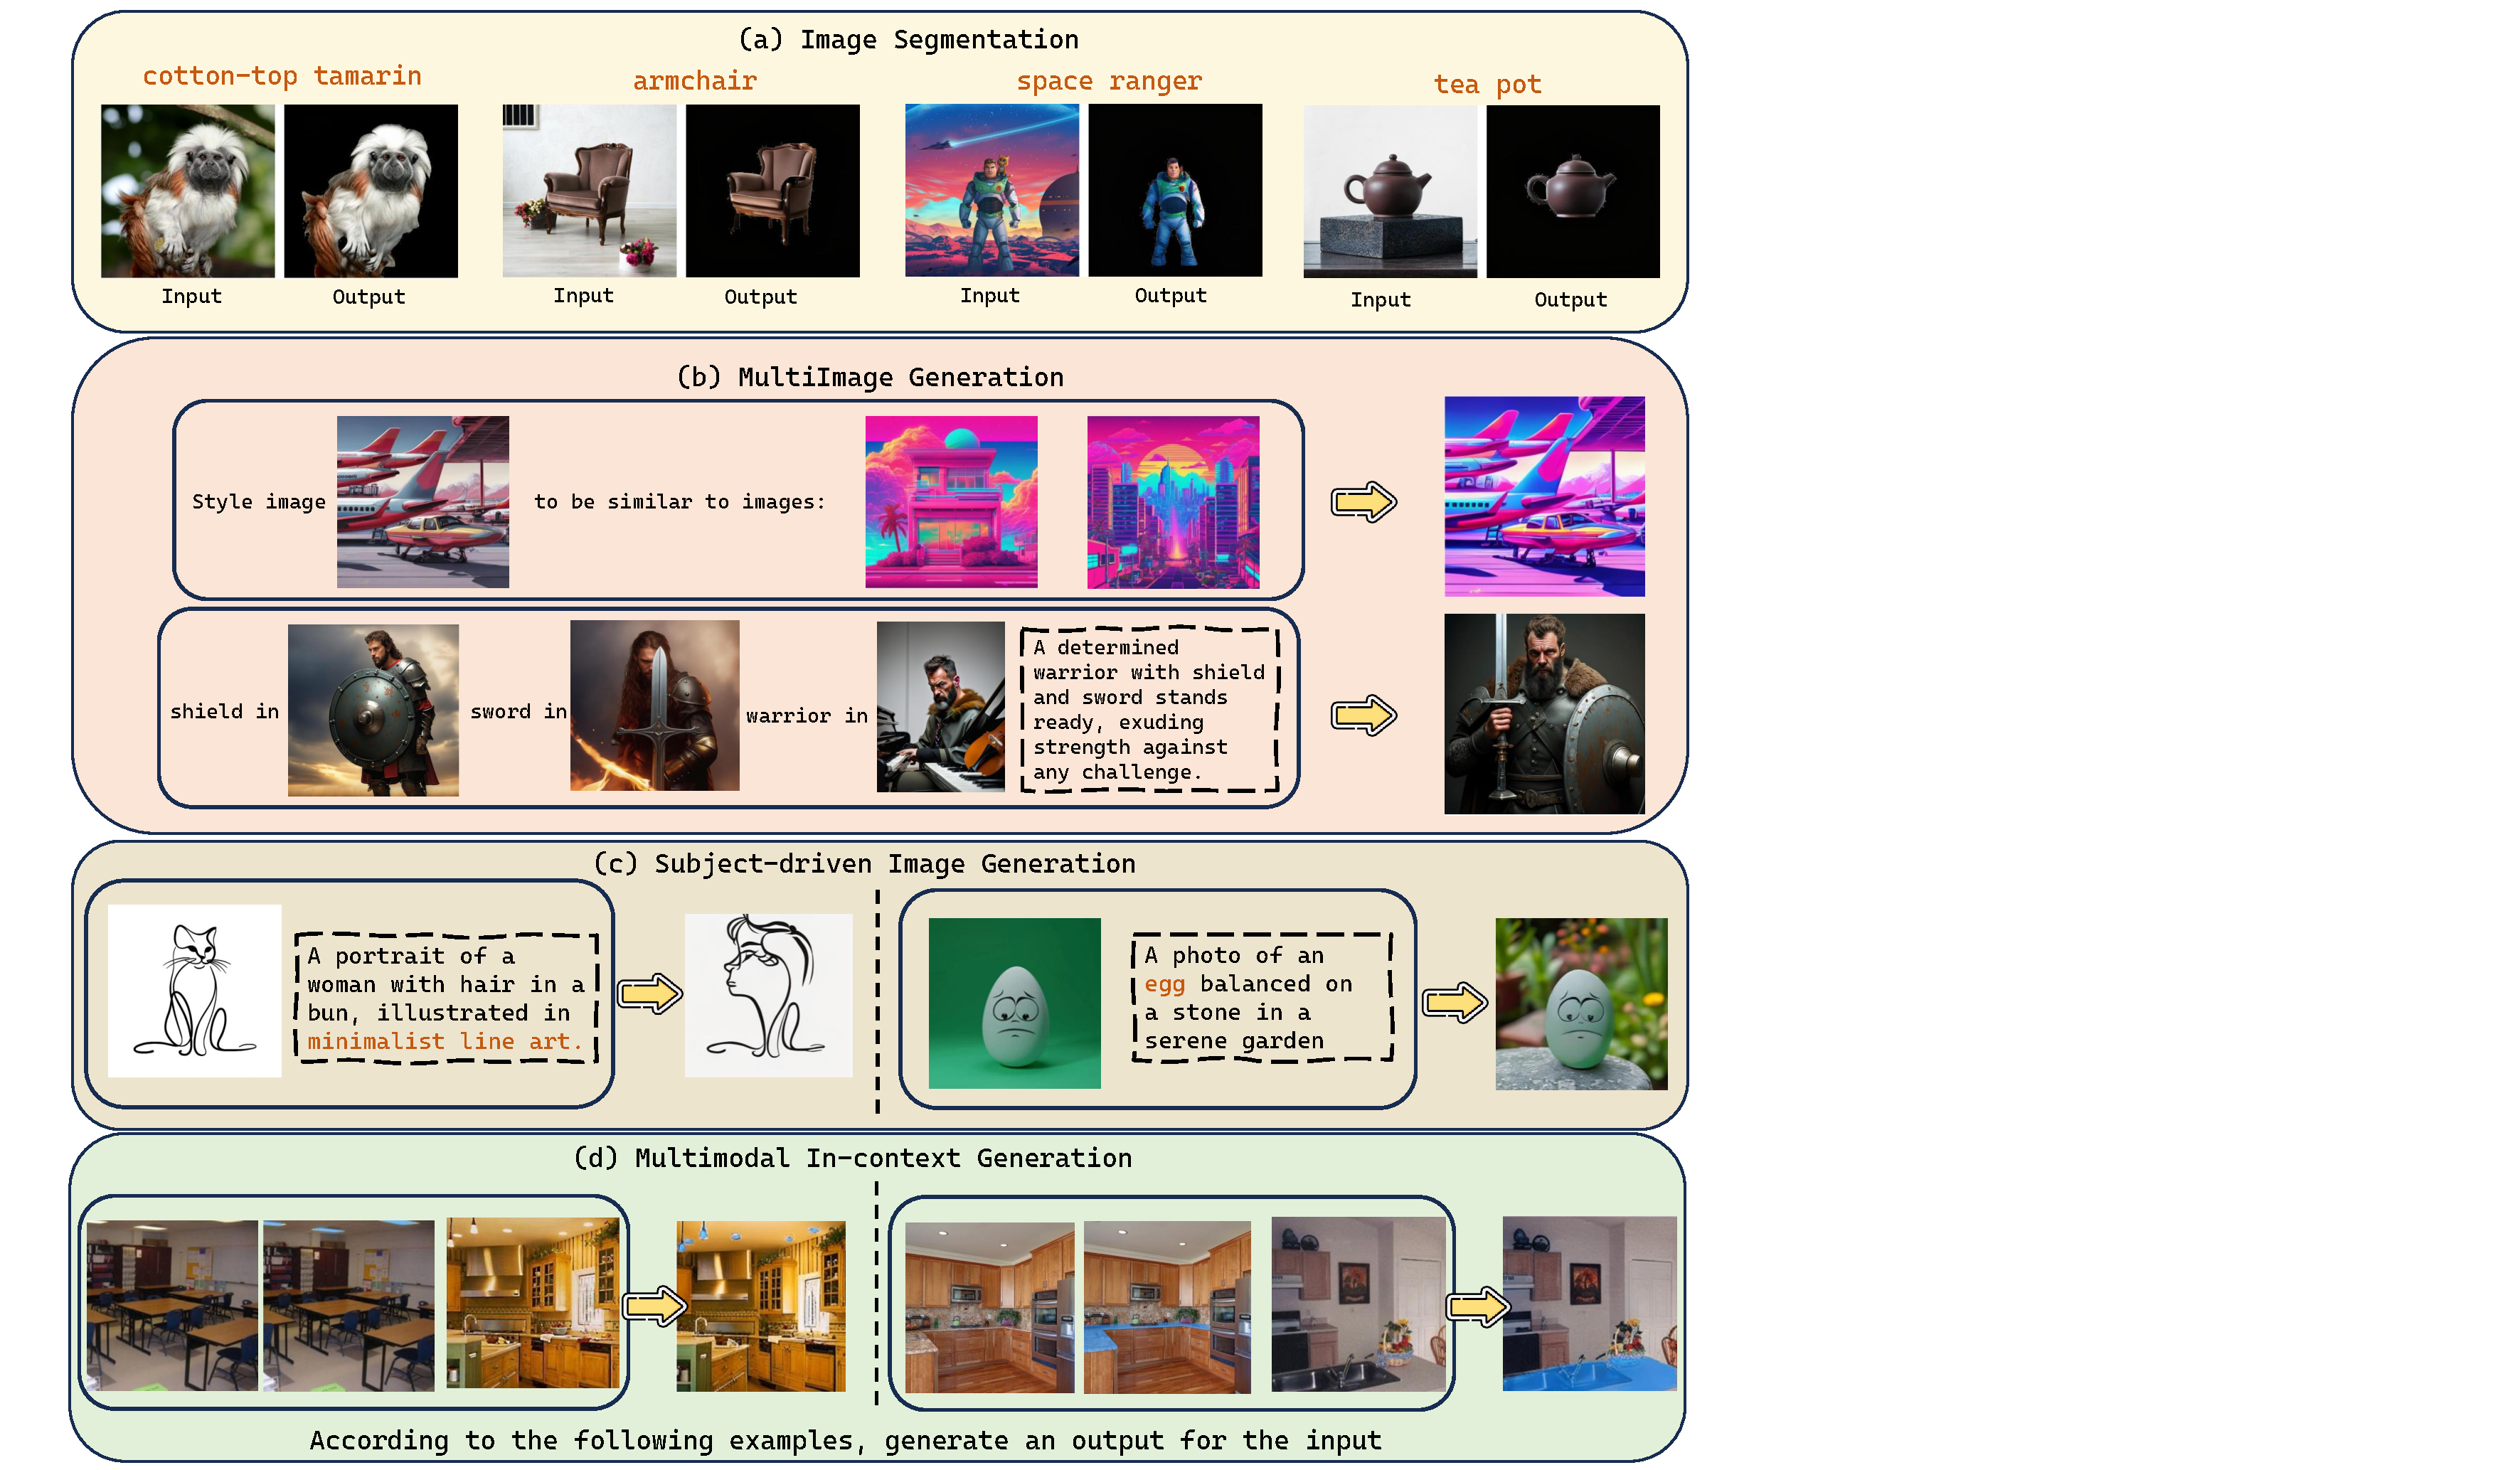
\includegraphics[width=1.0\textwidth]{figures/examples.pdf}
% 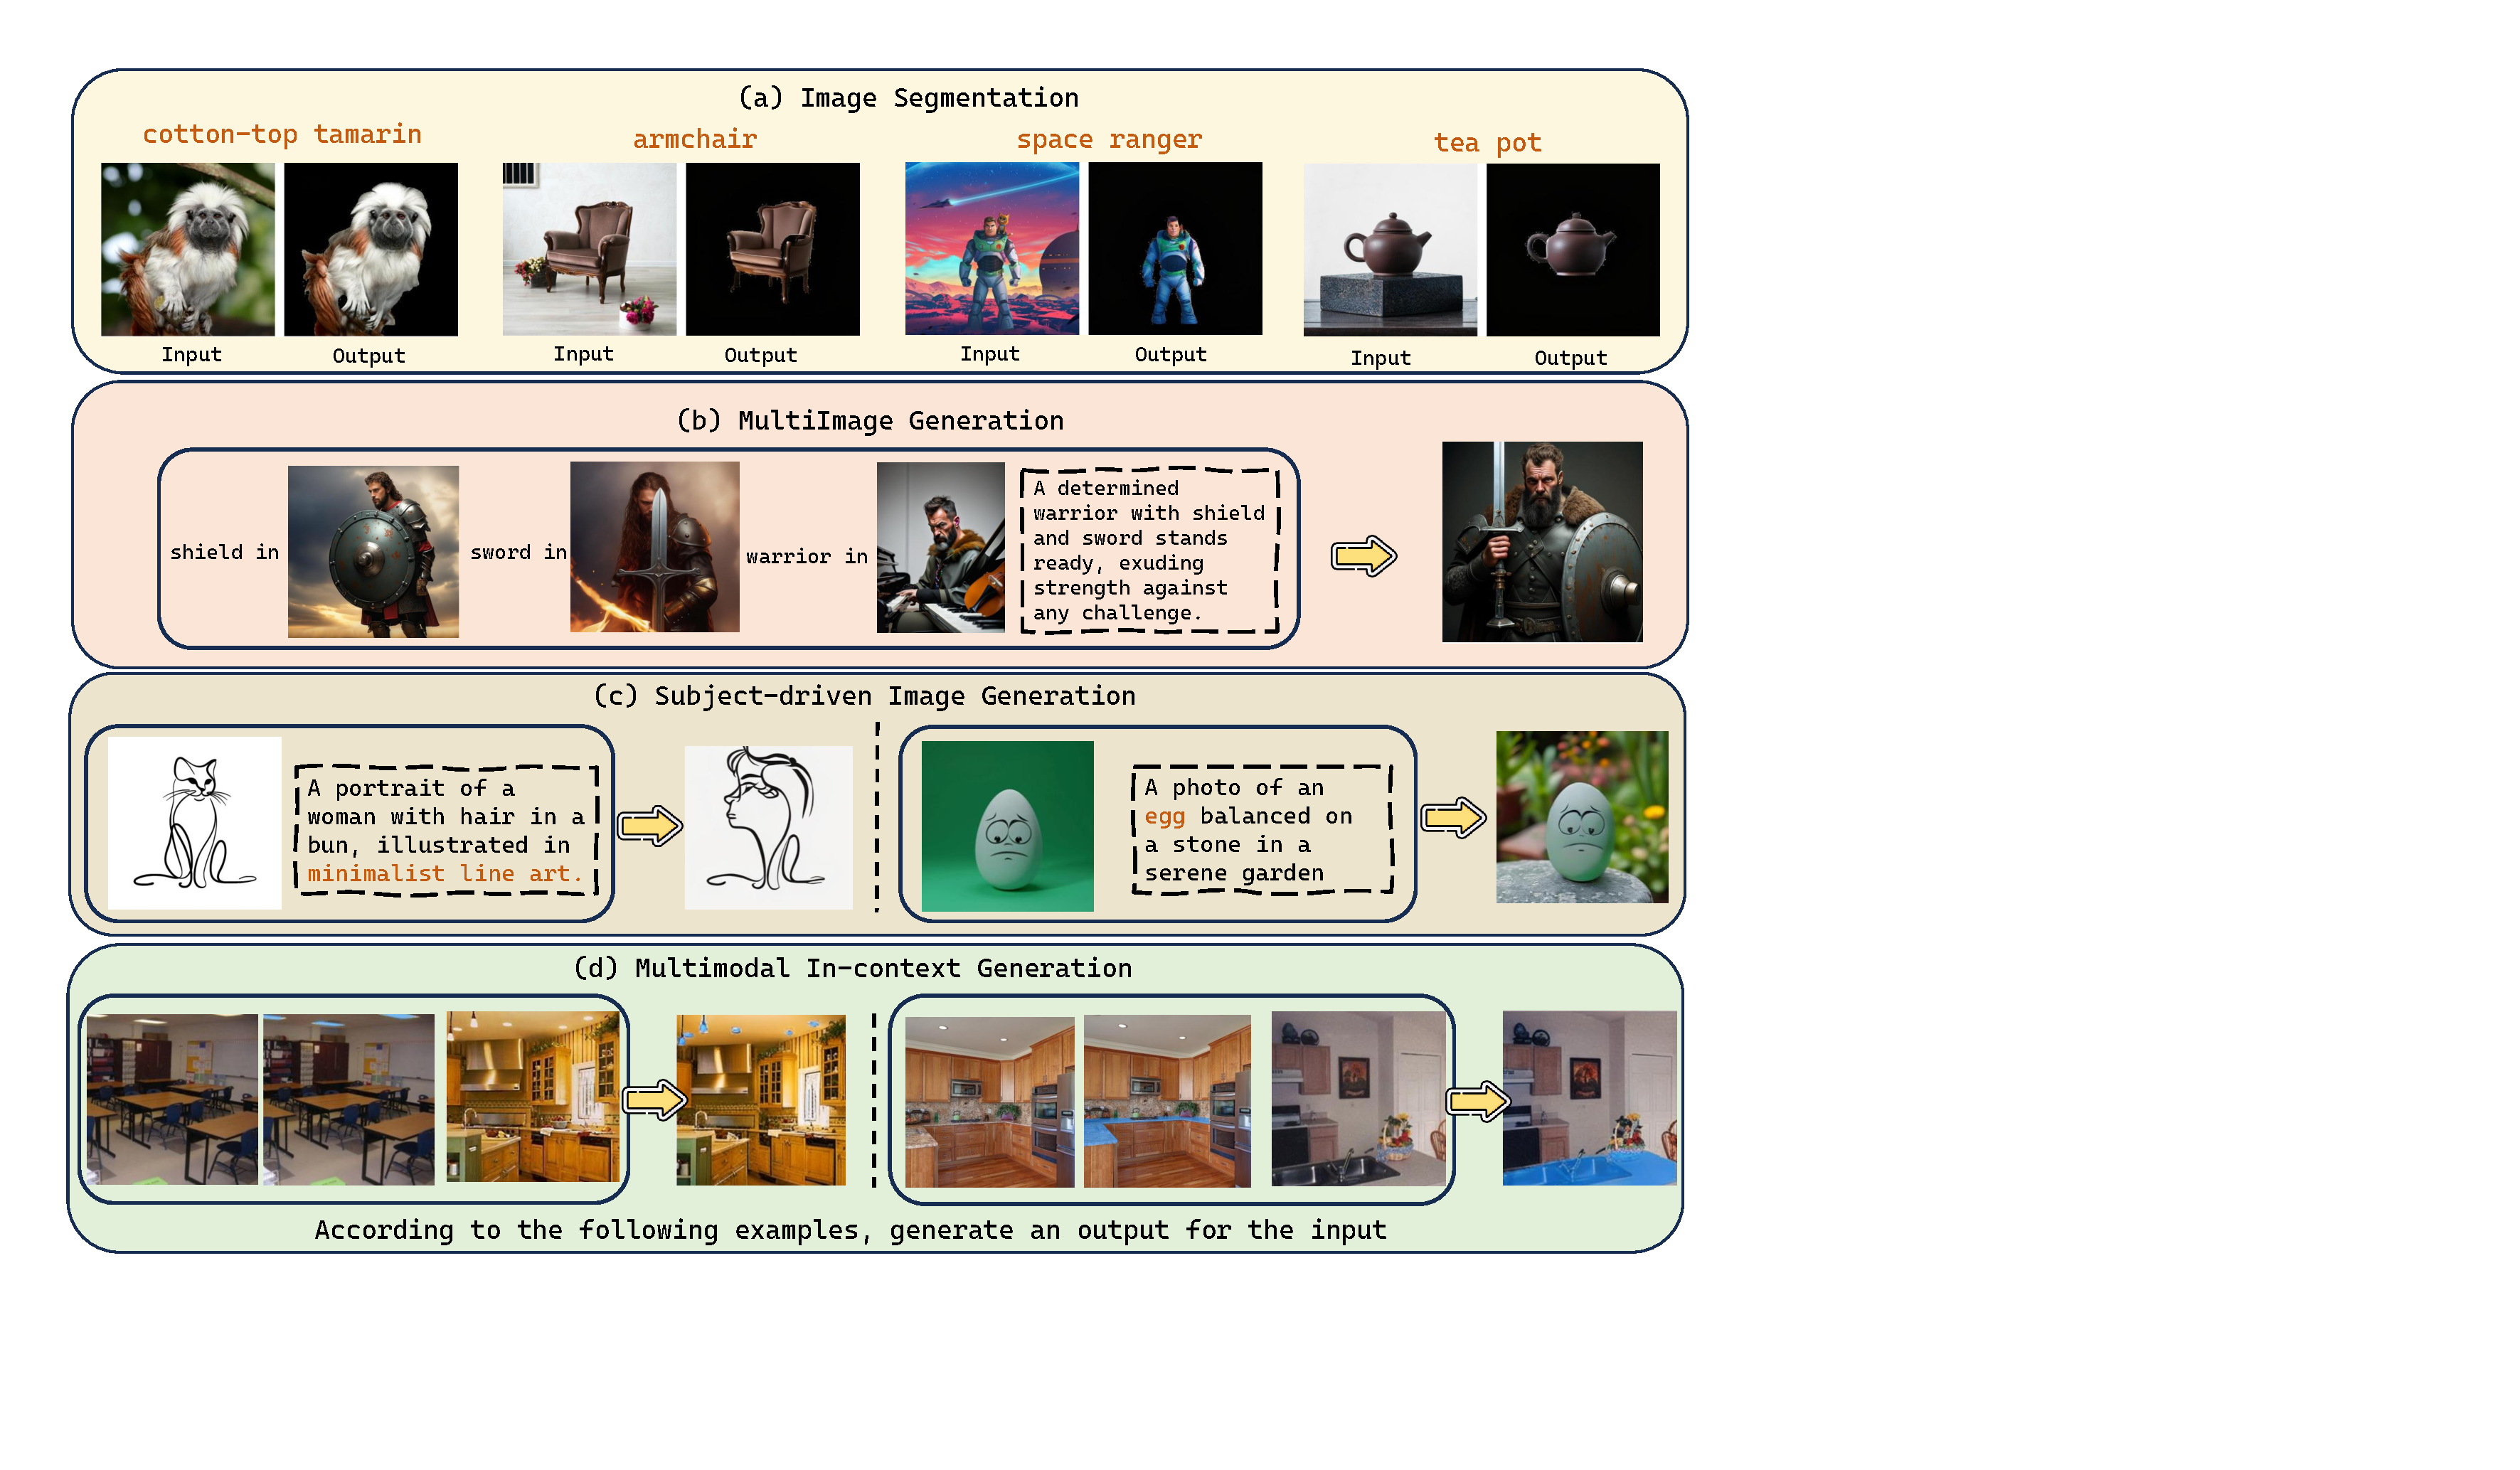
\includegraphics[width=0.7\textwidth]{figures/teasar.pdf}
% 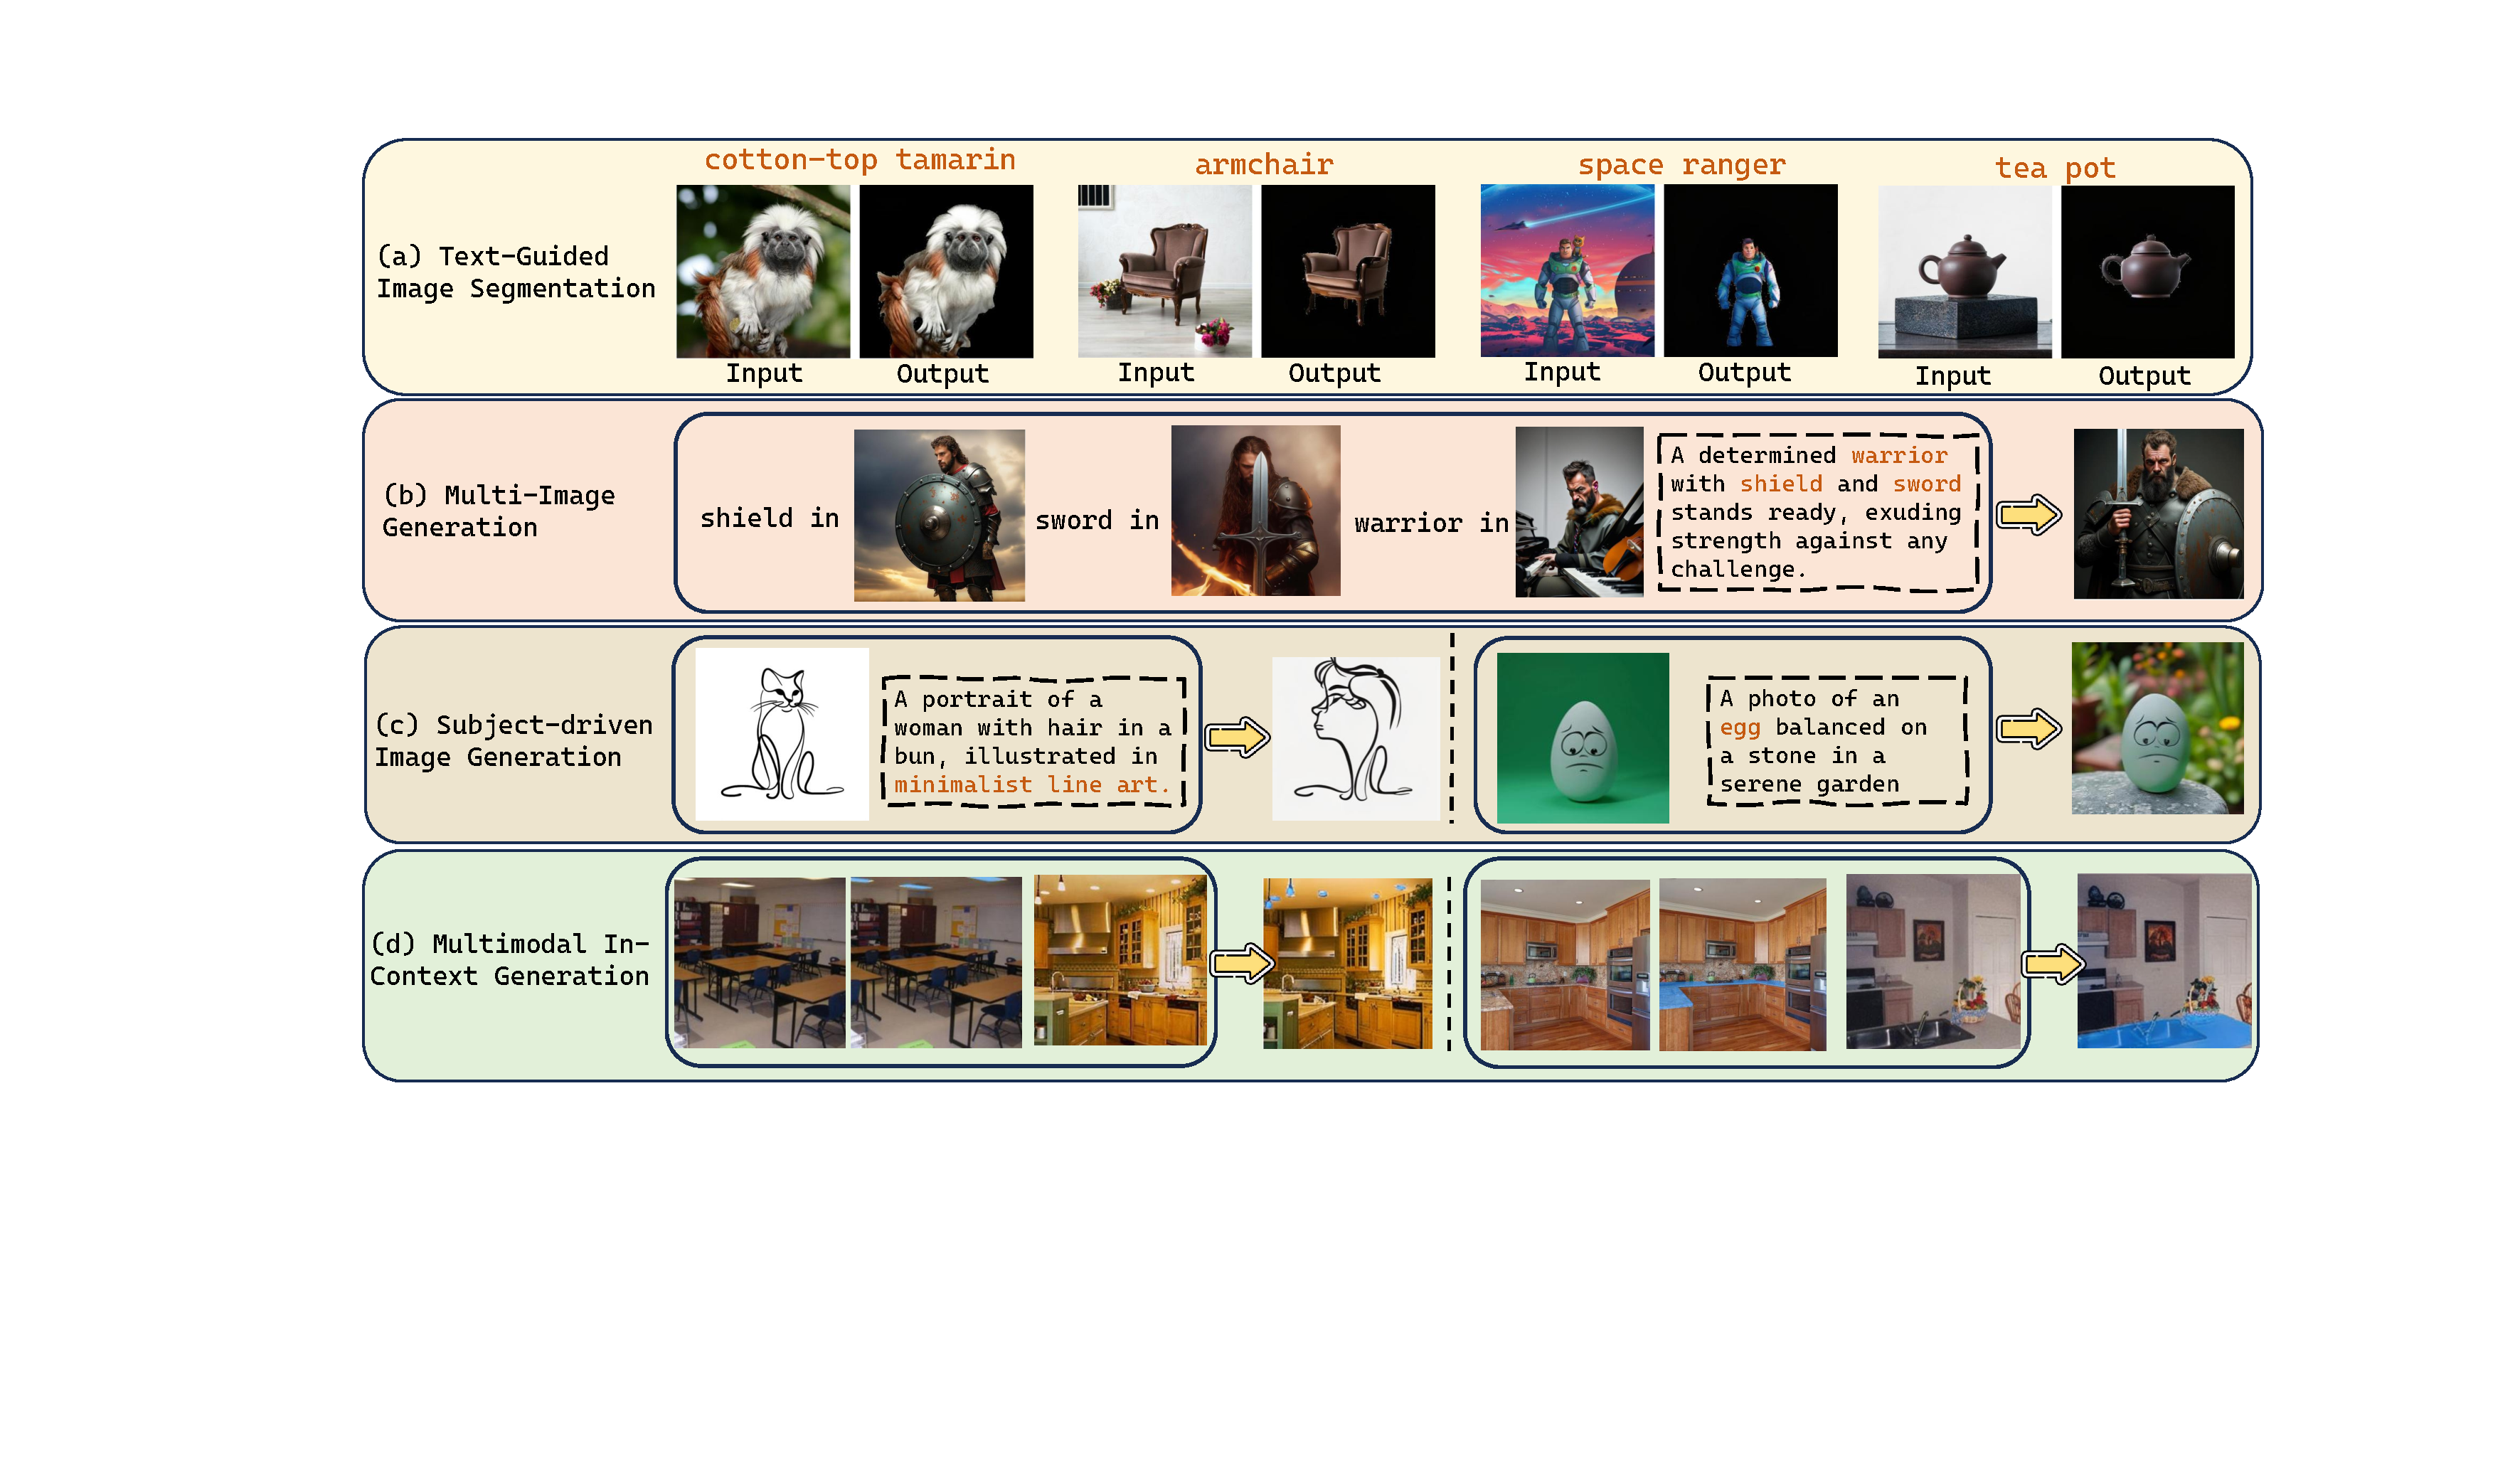
\includegraphics[width=0.9\textwidth]{figures/teasarv2.pdf}
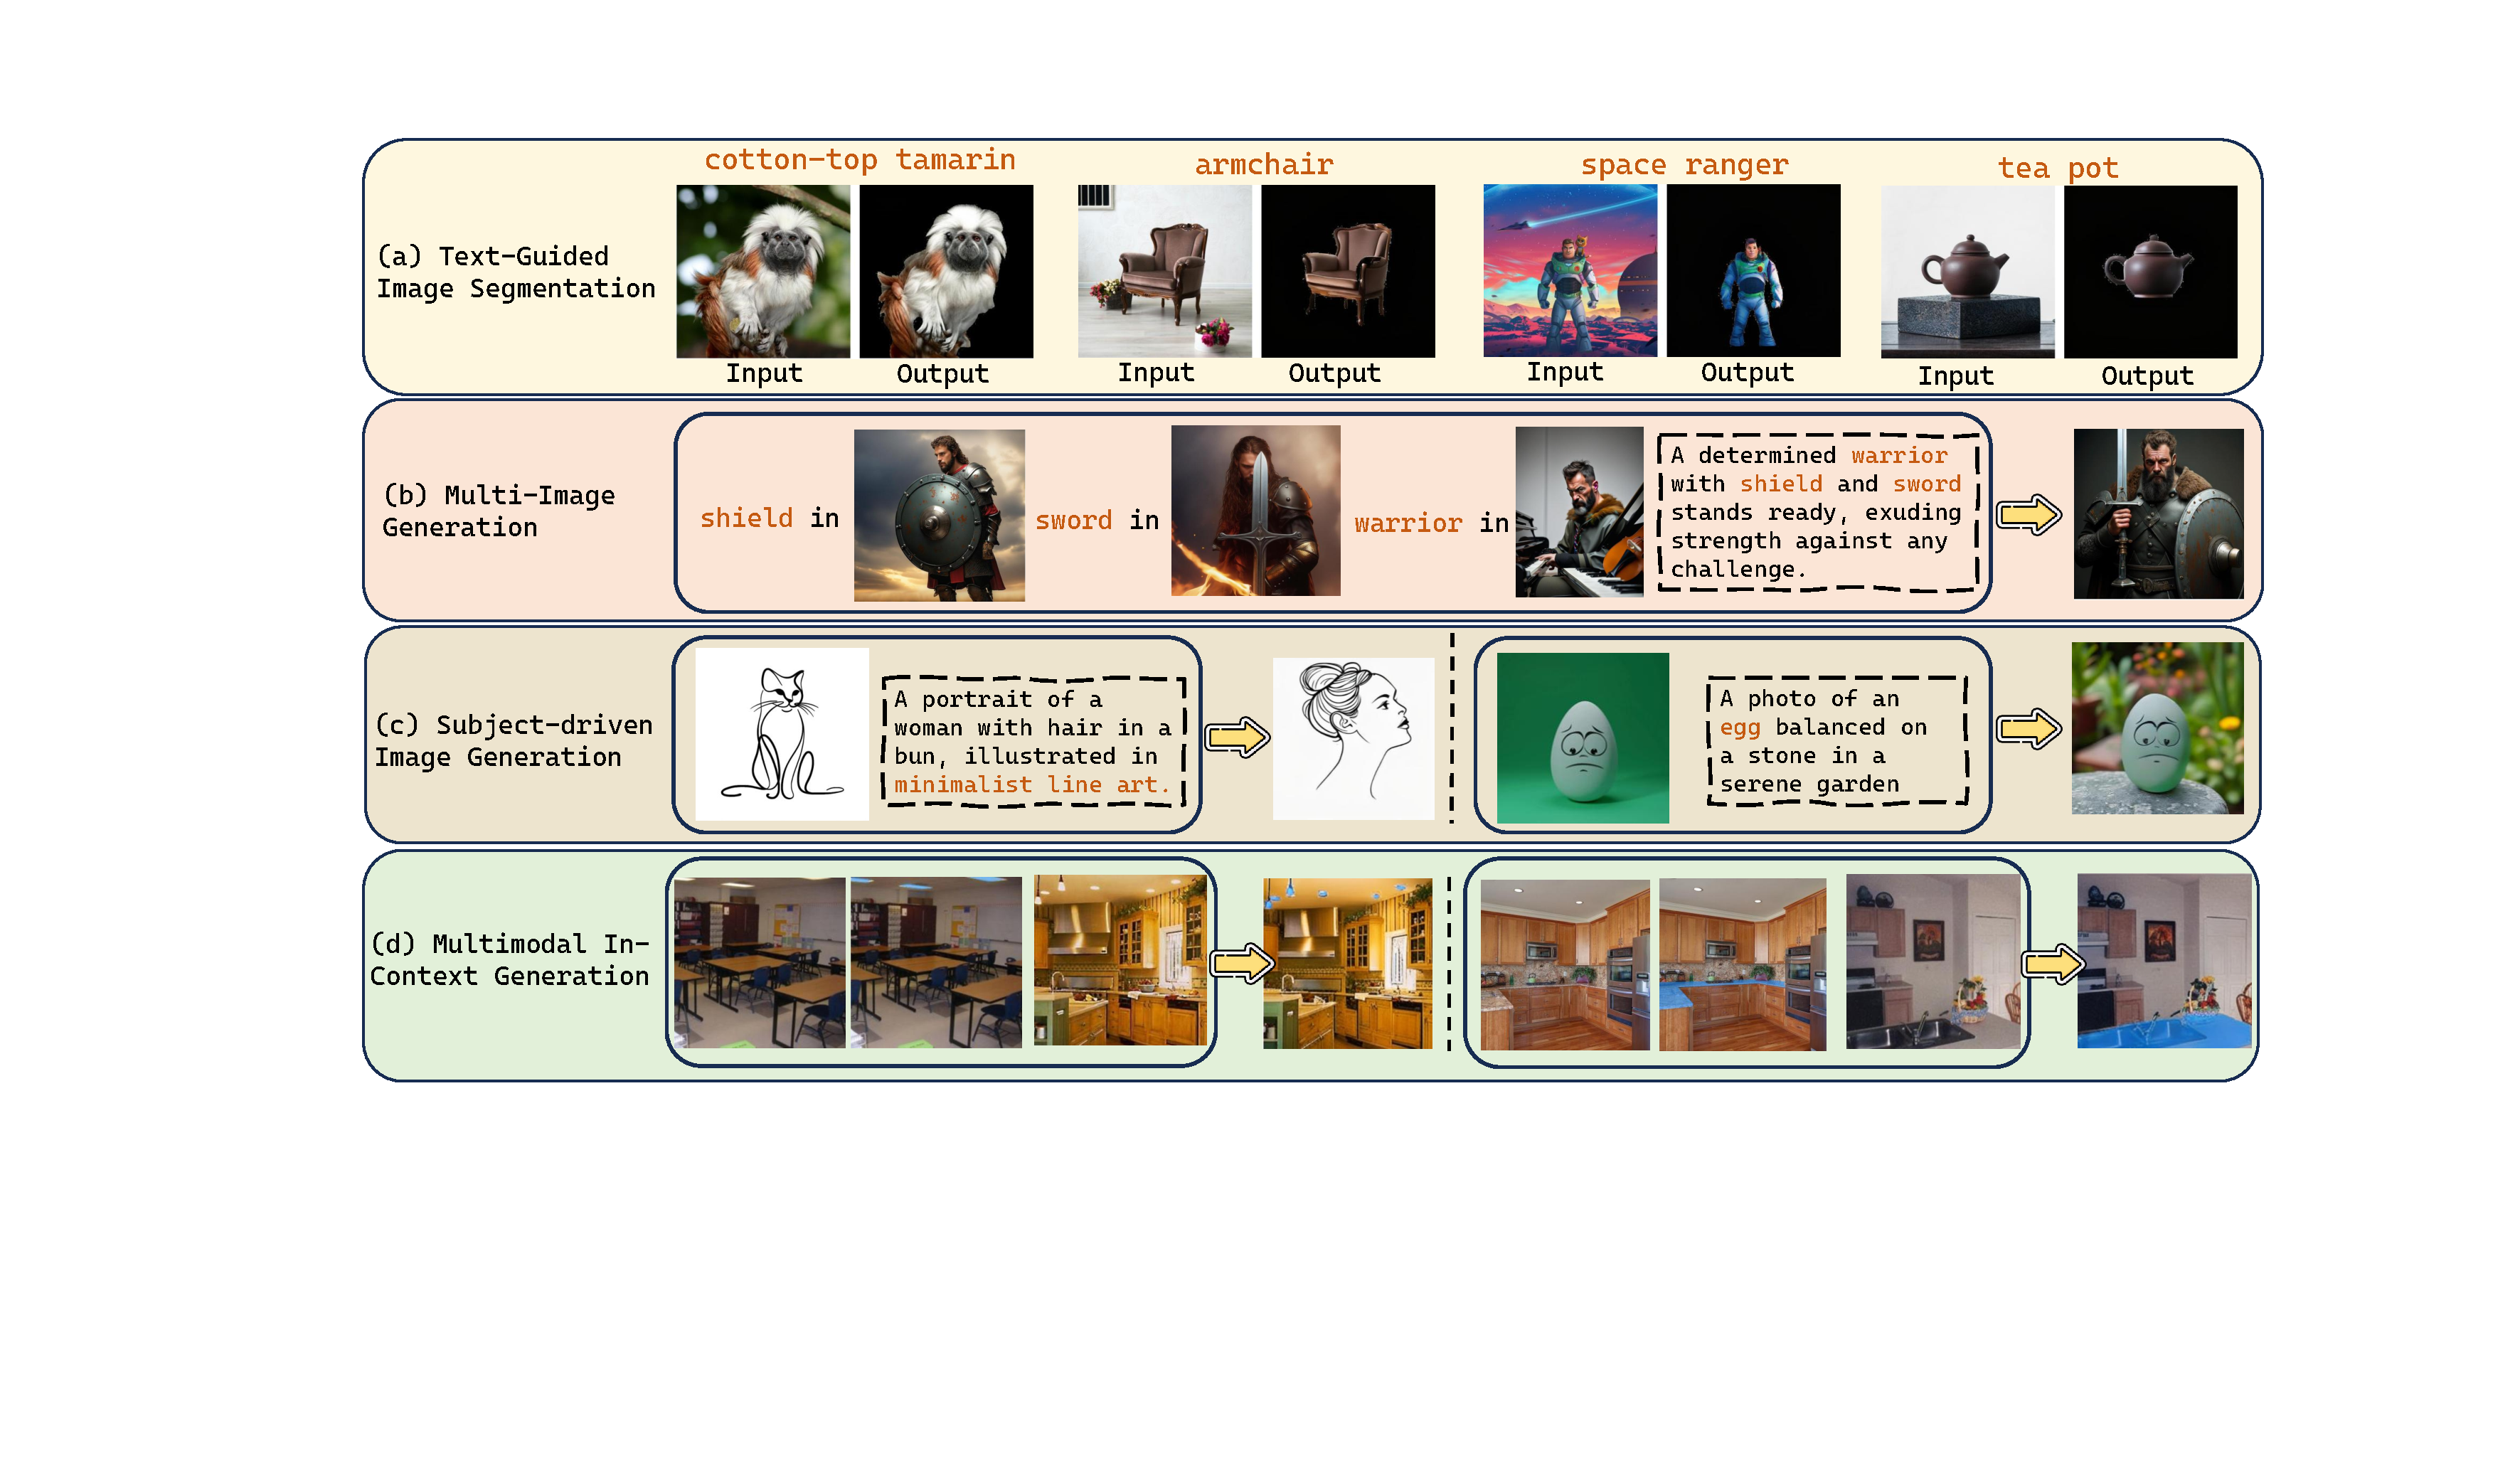
\includegraphics[width=0.9\textwidth]{figures/teasarv3.pdf}
\caption{Versatile applications built on \model after simply fine-tuning on corresponding datasets.
% , including (a) image segmentation, (b) multi-image generation, (c) subject-driven image generation, and (d) multimodal in-context learning image generation
}
\label{fig:examples}
\end{figure*}
\end{abstract}